%ACM journals format:
\documentclass[prodmode,acmtodaes]{acmsmall} 
\usepackage[ruled]{algorithm2e}
\renewcommand{\algorithmcfname}{ALGORITHM}
\SetAlFnt{\small}
\SetAlCapFnt{\small}
\SetAlCapNameFnt{\small}
\SetAlCapHSkip{0pt}
\IncMargin{-\parindent}

%Springer DAES format below:
%\documentclass[runningheads,a4paper]{llncs}
%\usepackage{amssymb}
%\setcounter{tocdepth}{3}
%\usepackage{graphicx}

% Metadata Information
%\acmVolume{9}
%\acmNumber{4}
%\acmArticle{39}
%\acmYear{2010}
%\acmMonth{3}

% Document starts
\begin{document}

% Page heads
\markboth{I. Filippopoulos et al.}{Data Interleaving and Memory Mapping on VLIW architectures}

% Title portion
\title{Integrated Optimization Methodology for Data Interleaving and Memory Mapping Exploration on VLIW architectures}
\author{IASON FILIPPOPOULOS
\affil{Norwegian University of Science and Technology}
NAMITA SHARMA 
\affil{Indian Institute of Technology Delhi}
FRANCKY CATTHOOR
\affil{IMEC}
PER GUNNAR KJELDSBERG
\affil{Norwegian University of Science and Technology}
PREETI PANDA
\affil{Indian Institute of Technology Delhi}
}

\begin{abstract}
This work presents a methodology for efficient exploration of data interleaving and data-to-memory mapping options for SIMD (Single Instruction Multiple Data) platform architectures.
The system architecture includes VLIW (Very Long Instruction Word) function units and a reconfigurable clustered memory. 
The scope is the reduction of the overall energy consumption by increasing the utilization of the function units and decreasing the number of memory accesses.
The presented methodology is tested using a number of benchmark applications with irregularities on their access scheme.
Potential gains are calculated based on the energy models both for the processing and the memory part of the system.
\end{abstract}

\category{D.2.2}{Design Tools and Techniques}{Design, Methodologies}
\category{B.7.1}{Types and Design Styles}{Memory Technologies, Design}
\category{B.8.2}{Performance Analysis and Design Aids}{}

\terms{Design, Algorithms, Performance}

\keywords{Data interleaving, single instruction multiple data (SIMD), system scenarios, design space exploration, memory reconfiguration}

%\acmformat{Iason Filippopoulos, Namita Sharma, Francky Catthoor, Per Gunnar Kjeldsberg, Preeti Panda, 2015. Integrated Optimization Methodology for Data Interleaving and Memory Mapping Exploration on VLIW architectures.}

%\begin{bottomstuff}
%Author's addresses: Iason Filippopoulos {and} Per Gunnar Kjeldsberg, Department of Electronics and Telecommunications, Norwegian University of Science and Technology (NTNU), Trondheim, Norway; Namita Sharma  {and} Preeti Panda, Department of Computer Science and Engineering, Indian Institute of Technology Delhi, New Delhi, India; Francky Catthoor, IMEC, Leuven, Belgium.
%\end{bottomstuff}

\maketitle

\section{Introduction}

The goal of this work is to improve both the performance and the energy consumption for data intensive applications. 
We focus on single instruction, multiple data (SIMD) architectures and deal with applications that have irregularities on their access scheme. 
SIMD architectures can potentially increase the performance of an application, providing that the utilization of them is high. 
However, applications with irregular access patterns do not provide compact sequences of data that are suitable for high utilization. 
Hence the performance is lower than expected. 
In order to improve the performance a systematic exploration of the interleaving options for application's data is needed. 

The energy consumption can be divided into two parts, namely the processing and the memory subsystem. 
The energy needed for processing depends mainly on the utilization of the FUs and any potential stalls, if the memory cannot provide data on the needed rate.
The interleaving exploration can increase the utilization of the processing subsystem and reduce time penalties for data loading.   
The energy consumption on the memory subsystem is affected by the number of memory accesses and the energy per access. 
Again, the memory architecture and the data-to-memory mapping decisions have a great impact on both the number of accesses and the energy per access.

\section{Motivational Example}
\label{sec:motivational}

A large number of papers have demonstrated the importance of the memory organization to the overall system energy consumption. 
As shown in \cite{Gonzalez1996} memory contributes around 40\% to the overall power consumption in general purpose systems. 
Especially for embedded systems, the memory subsystem accounts for up to 50\% of the overall energy consumption \cite{Che09} and the cycle-accurate simulator presented in \cite{Ben99} estimates that the energy expenditures in the memory subsystem range from 35\% up to 65\% for different architectures. 
The breakdown of power consumption for a recently implemented embedded system presented in \cite{Hul11} shows that the memory subsystem consumes more than 40\% of the leakage power on the platform. 
According to \cite{tcm}, conventional allocation and assignment of data done by regular compilers is suboptimal. 
Performance loss is caused by stalls for fetching data and data conflicts for different tasks, due to the limited size of memory and the competition between tasks. 

To illustrate the sub-optimal utilization of SIMD architectures using conventional allocation and assignment of data, the simple example of Alg.~\ref{alg:motivation} is used.
In this example, we assume that the desired result is always the sum of 4 elements from arrays \textit{A, B, C and D}. 
The access pattern shows an irregularity, as a result of the iteration index.
For every group of four sequential array elements, there is only one used for the calculation of the result and the other three are skipped.
An intuitive interleaving optimization is the interleaving of the arrays \textit{A, B, C and D}, in order to generate sequences of elements that are all useful on the calculation of the \textit{result} variable. 
A full interleaving exploration could reveal several options to produce larger sequences of array elements that are needed during the execution of Alg.~\ref{alg:motivation}.
For example, the interleaving of every fourth line within the combined array ($A\vert B\vert C\vert D$) result in a sequence of 8 accessed elements.

\begin{algorithm}[t]
\SetAlgoNoLine
\For{($i = 0; i < N; i+4$)}{
        ${result(i) = A(i) + B(i) + C(i) + D(i)}$\;
}
\caption{Motivational Example Algorithm}
\label{alg:motivation}
\end{algorithm}

The data-to-memory mapping is presented in Fig.~\ref{motivation}. 
The memory architecture consists of four memory banks and the overall memory size is enough to fit the four arrays.
The conventional approach maps each array in a separate bank.
If the four arrays are interleaved, the mapping distributes the data through the banks.
The first four elements are respectively from arrays A, B, C and D and so forth.
As a result only one forth of the array A can be found on the first bank in contrast to the non-interleaving case, in which the whole array A is mapped on the first bank.

\begin{figure}
\centering
	\label{motivation}
	\caption{Data-to-memory mapping for motivational example}
	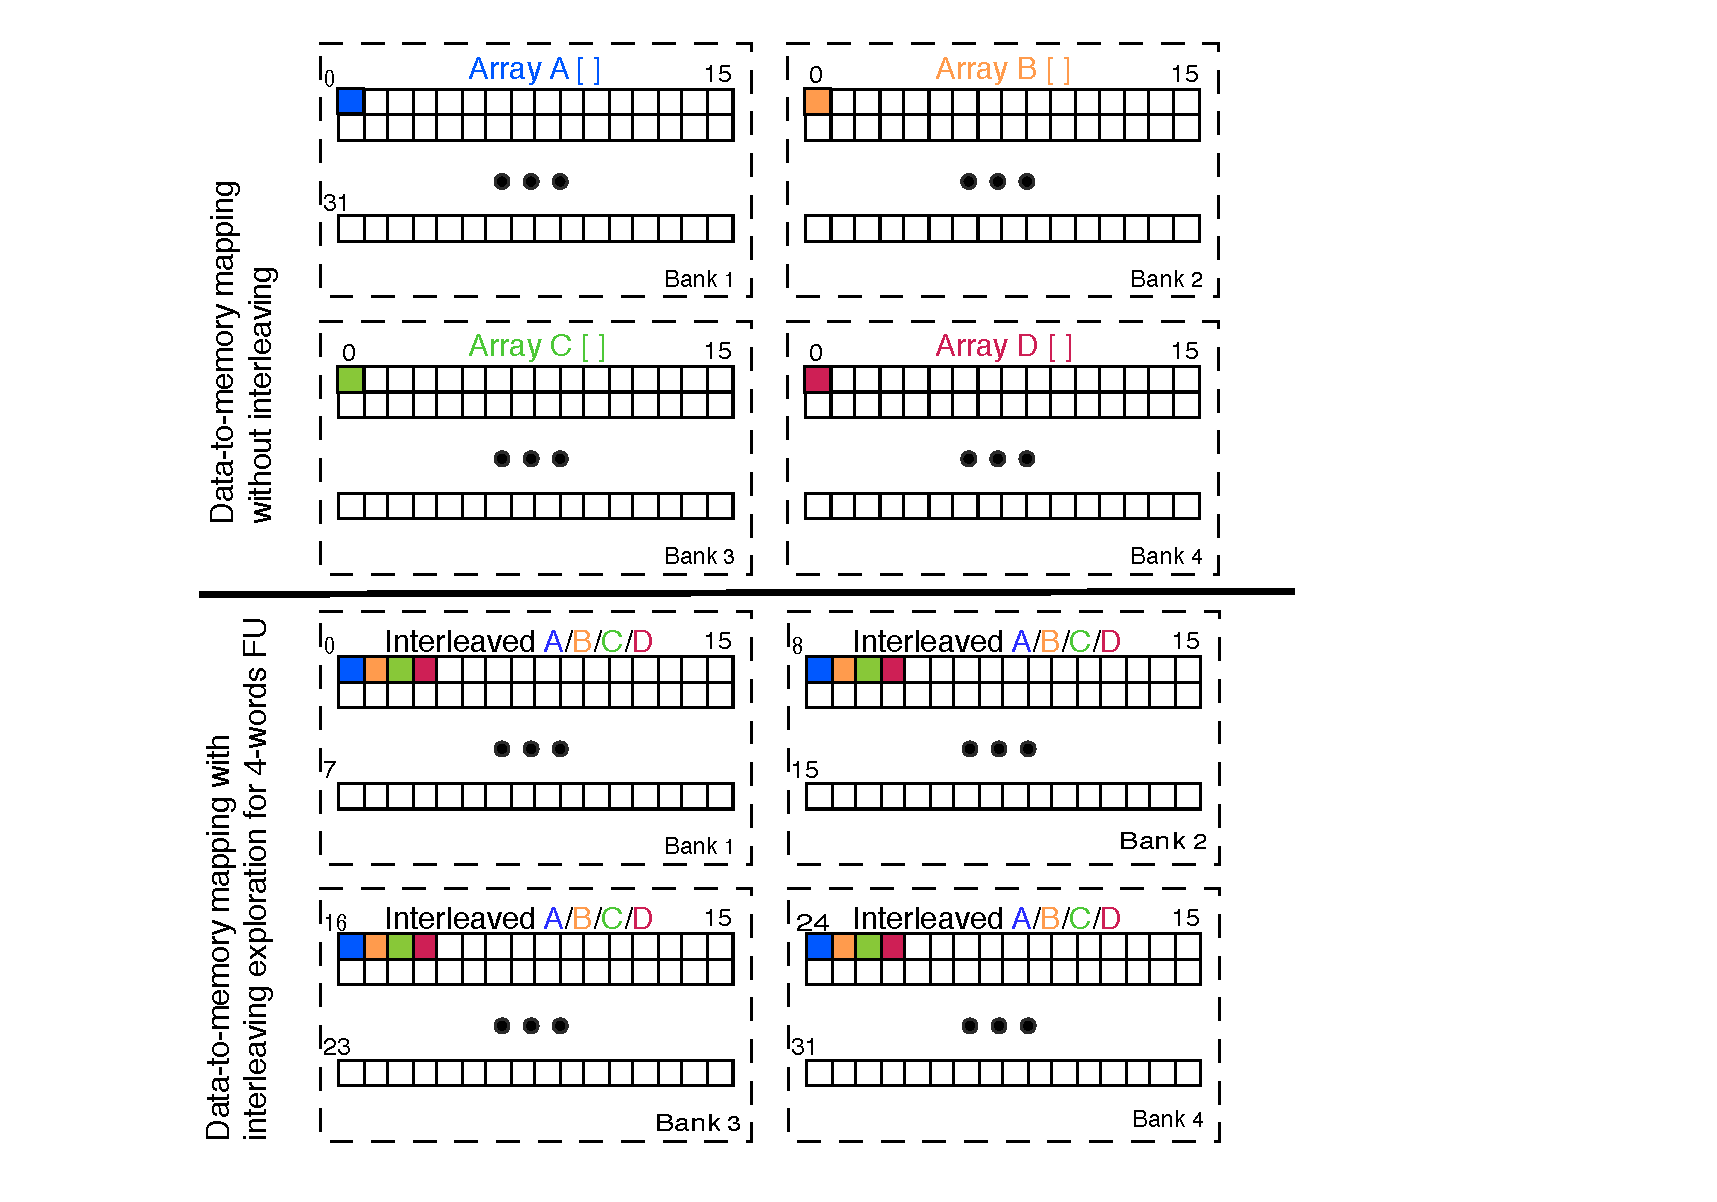
\includegraphics[scale = 0.5]{Images/motivation.eps}
\end{figure}

A quick estimation for the difference in the energy consumption between the two approaches can be calculated using a simple energy model for the system.
We can assume a system architecture with an ADD FU that performs operations over 4 words at a time and a memory to processor path that has a width of 4 words. 
Each array element is assumed to have the size of one word.
The register file at the processor can only store the iteration variable $i$ and 5 words, which are the variables result, A, B, C and D.
Without interleaving of data the number of memory accesses for each loop iteration is 4, because the elements $A(i)$, $B(i)$, $C(i)$ and $D(i)$ are stored in different memory banks.
Thus, the energy consumption for reading is 75\% lower when the data are interleaved.
The performance is also higher as there are 75\% less memory accesses.
The energy consumption due to memory leakage is also lower, as the access time for the memory and the execution time of the algorithm are shorter.

\section{Related work}

The current work combines and expands the interleaving exploration presented in \cite{sharma2013data} and the data to memory mapping methodology presented in \cite{filippopoulos2013exploration}. Data layout optimizations aim to arrange data in memory with the objective of improving system performance and energy through means such as reduced memory access count or reduced cache misses. Several more generic data layout techniques have been explored by researchers at various levels in the memory hierarchy. But these are not well matched to our context of LTE optimisations. In particular, Cache partitioning [4], a layout technique for arrays, maps each array to different cache partitions to reduce conflicts. Kulkarni et al. [5] addressed the problem for cache miss reduction by evaluating the tiling size for arrays and merging the arrays appropriately for each loop nest. Memory Hierarchy Layer Assignment (MHLA), an optimization methodology for data memory hierarchy [6], determines for each data set an appropriate layer in the hierarchy and type of memory (single/dual port) taking data re-use into account. The strategy in [7] partitions the variables to Scratch Pad Memory and DRAM in a way that interference among different variables is minimized. To the best of our knowledge, no work has been presented yet for an efficient data layout for LTE. And the cache-oriented general techniques proposed earlier by researchers [8] do not find a straightforward application in our context, where the target system hardware consists of a coarse grained re-configurable array (CGRA) of SIMD functional units and vector registers.

The memory allocation problem has been studied before. 
However, we extend state of the art by proposing a more generic approach, which is also suitable for applications with input driven dynamic behaviour. 
The authors in \cite{Ben00b} present a methodology to generate a static application-specific memory hierarchy. 
Later, they extend their work in \cite{Ben00c} to a reconfigurable platform with multiple memory banks. 
However, our work differentiates by proposing a more generic and application agnostic methodology and employing the use of system scenarios, in order to efficiently handle a wider range of dynamic application characteristics. 

Several techniques for designing energy efficient memory architectures for embedded systems are presented in \cite{Mac02}. 
The current work differentiates by employing a platform that is reconfigurable at run-time. 
In \cite{Pgk01} a large number of data and memory optimisation techniques, that could be dependent or independent of a target platform, are discussed. 
Again, reconfigurable platforms are not considered.

Energy-aware assignment of data to memory banks for several task-sets based on the MediaBench suit of benchmarks is presented in \cite{Mar03}. 
Low energy multimedia applications are discussed also in \cite{Chu02} with focus on processing rather than the memory platform. 
Furthermore, both \cite{Mar03} and \cite{Chu02} base their analysis on use case situations and do not incorporate sufficient support for very dynamically behaving application codes. 
System scenarios alleviate this bottleneck and enable handling of such dynamic behaviour. 
In addition, the current work explores the assignment of data to the memory and the effect of different assignment decisions on the overall energy consumption.

The authors in \cite{abraham1999automatic}, \cite{jacob1996analytical} and \cite{li1999hardware} present methodologies for designing memory hierarchies.
Design methods with main focus on the traffic and latencies in the memory architecture are presented in \cite{chen1999loop}, \cite{grun2000mist}, \cite{jantsch1994hardware} and \cite{passes1995multi}.
Improving memory energy efficiency based on a study of access patterns is discussed in \cite{kandemir2001improving}.
Application specific memory design is a research topic in \cite{schmit1997synthesis}, while memory design for multimedia applications is presented in \cite{oshima1997high}.
The current work differentiates by introducing the concept of system scenarios that supports the dynamic handling of application's requirements, although the data mapping is static inside each scenario. 

An overview of work on system scenario methodologies and their application are presented in \cite{Gheorghita2007}. 
In \cite{Fil12} extensions towards a memory-aware system scenario methodology are presented and demonstrated using theoretical memory models and two target applications. 
This work is an extension both in complexity and accuracy of the considered memory library and on the number of target applications. 

Furthermore, the majority of the published work focus on control variables for system scenario prediction and selection. 
Control variables can take a relatively small set of different values and thus can be fully explored. However, the use of data variables \cite{Elena2010} is required by many dynamic systems including the majority of multimedia applications. 
The range of possible values for data variables is wider and makes full exploration impossible. 

Authors in \cite{Pal06} present a technique to optimise memory accesses for input data dependent applications by duplicating and optimising the code for different execution paths of a control flow graph (CFG). 
One path or a group of paths in a CFG form a scenario and its memory accesses are optimised using global loop transformations (GLT). 
Apart from if-statement evaluations that define different execution paths, they extend their technique to include while loops with variable trip count in \cite{Pal06b}. 
A heuristic to perform efficient grouping of execution paths for scenario creation is analysed in \cite{Pal07}. 
Our work extends the existing solutions towards exploiting the presence of a distributed memory organisation with reconfiguration possibilities.

Reconfigurable hardware for embedded systems, including the memory architecture, is a topic of active research. 
An extensive overview of current approaches is found in \cite{Garcia}. 
The approach presented in this paper differentiates by focusing on the data-to-memory assignment aspects in the presence of a platform with dynamically configurable memory blocks. 
Moreover, many methods for source code transformations, and especially loop transformations, have been proposed in the memory management context. 
These methods are fully complementary to our focus on data-to-memory assignment and should be performed prior to our step. 

\section{System Design Exploration Workflow}

The overall flow of this work is presented in Fig.\ref{workflow}. 
The first step of the methodology is the analysis of the application code. 
The methodology is applicable to any application.
However the applications that can benefit from the methodology are the ones with irregular access patterns.
The second step is the interleaving exploration, which explores all different option for re-arrangement of the data.
The result of the interleaving is a set of data with a reduced number of holes.
The next step is the mapping of the interleaved data set to the clustered memory architecture.
The exploration space consists of different sizes and types of memory banks.

\begin{figure}
\centering
	\label{workflow}
	\caption{Methodology steps}
	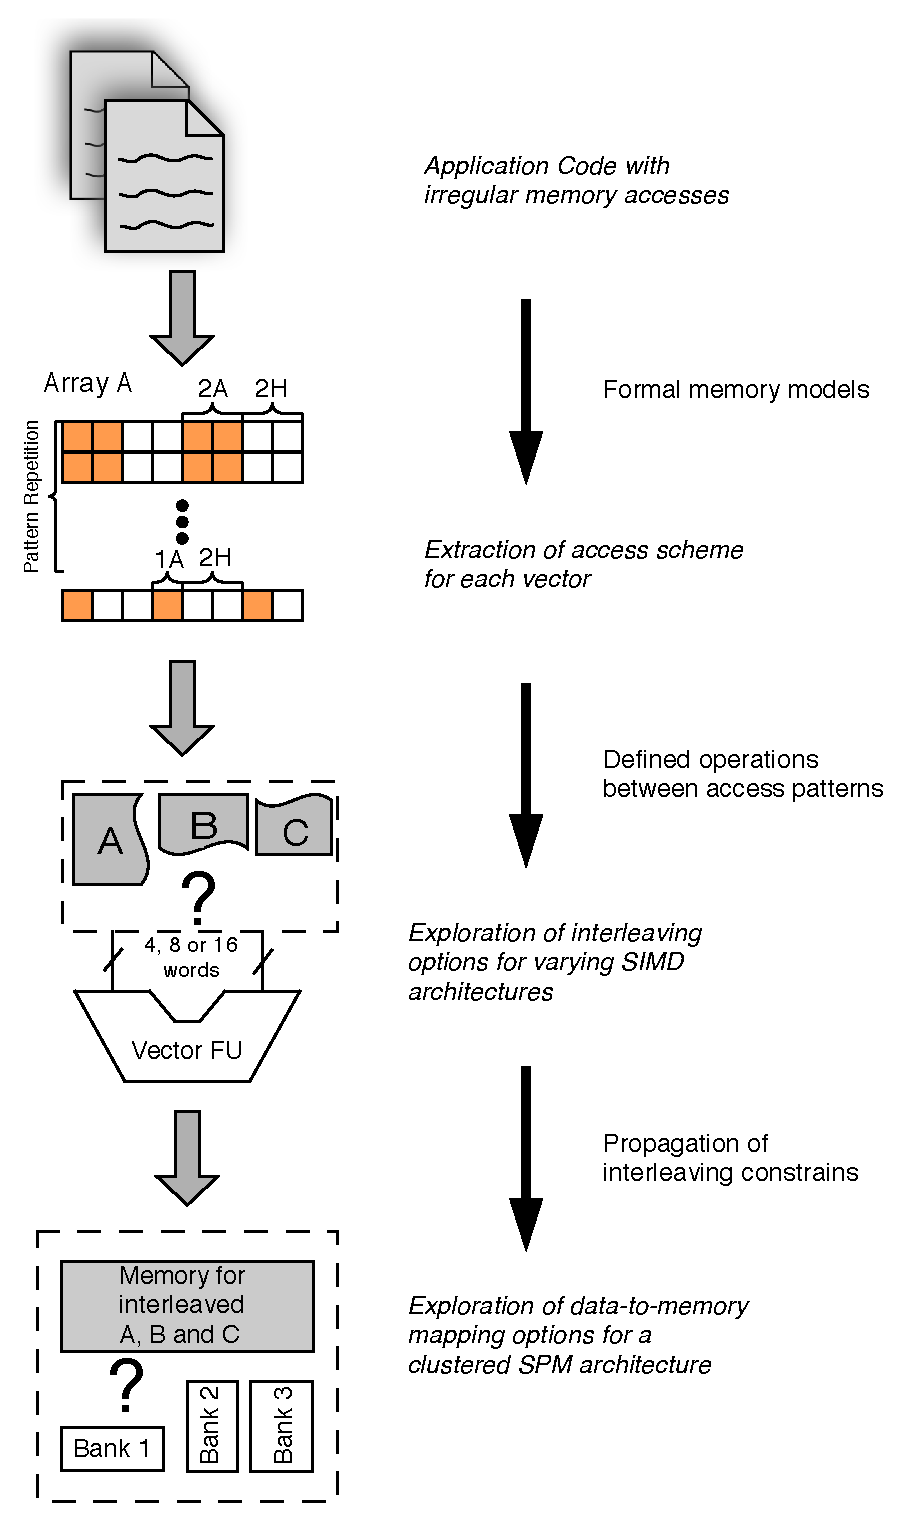
\includegraphics[scale = 0.5]{Images/Workflow.eps} 
\end{figure}

\subsection{Formal Model Representation of Access Pattern }

A representation model for the access pattern is employed in order to formally present each step of the methodology.


%\textit{Discussion about polyhedral and enumerative approaches}
%
%\textit{Analysis of A-H model based on Angeliki}
%
%\textit{Definition of algebra functions between access patterns}

\subsection{Data Interleaving Exploration}
Interleaving is a data layout transformation for combining the storage of multiple arrays, so that blocks of data from different arrays are stored contiguously, in order to achieve spatial locality in memory accesses.
By interleaving we are able to group the data to be accessed and thus reduce the number of memory accesses for loading them.
%\textit{Algorithm for exploring data interleaving}

\subsection{Data-to-Memory Mapping Exploration}

Given the input from the previous step, we explore the mapping of the interleaved data to the memory architecture.
A clustered memory organisation with up to five memory banks of varying sizes is explored. 
The limitation in the number of memory banks is necessary in order to keep the interconnection cost between the processing element (PE) and the memories constant through exploration of different architectures. 
The decision to use memory banks with varying sizes on the clustered memory organization increases the reconfiguration options and consequently the potential energy gains. 
In general, smaller memories are more energy efficient compared to larger memories banks. 
However, in some cases large memory banks are needed in order to fit the application data without the need for too many small memories causing complex interconnects. 
The goal is to use the most energy efficient banks to store the interleaved data.

\subsection{One way constraint propagation}

The decisions taken on the interleaving step affect the mapping options.
If the interleaving decisions lead to small compact sets of data, the mapping can be done on small energy efficient memory banks.
On the other hand, if the mapping exploration is performed first, the freedom for interleaving is reduced.
We split the decisions in two steps and the interleaving decisions are propagated as constraints on the mapping exploration phase. 

\section{Target Architecture}

%\textit{Analysis of architecture based on our previous papers}
A generic architecture is presented in Fig.\ref{arch}.
The methodology explores different interleaving and data to memory mapping options for this reconfigurable architecture.
The scratchpad memory consists of up to five memory banks. 
The optimal sizes are found based on the sizes of the data after the interleaving exploration.
The vector FU is assumed to perform instructions on multiple data.
The explored data lengths are 4, 8 and 16 words.
Each word is an array elements in our case. 

\begin{figure}
\centering
	\label{arch}
	\caption{Exploration options and system knobs depending on a general platform architecture}
	\includegraphics[scale = 0.5]{Images/Architecture.eps} 
\end{figure}

\subsection{Memory Models}

The dynamic memory organisation is constructed using commercially available SRAM memory models (MM).
For those models delay and energy numbers are derived from a commercial memory compiler.
In addition, experimental standard cell-based memories (SCMEM) \cite{Mei11}  are  considered for smaller memories due to their energy and area efficiency for reasonably small storage capacities, as argued in \cite{Mei10}. 
The standard cell-based memories are synthesized using Cadence RTL compiler for TSMC 40nm standard library. 
Afterwords, power simulations on the synthesized design are carried out using Synopsys PrimeTime, in order to obtain energy numbers.
Both MMs and SCMEMs can operate under a wide range of supply voltages, thus support different operating modes that provide an important exploration space.

\subsection{Function Unit Models}

We have used an extension of the DRESC compiler framework [10] for mapping the reference application to a CGRA architecture.
The CGRA part comprises four SIMD enabled functional units (FUs) and a central vector register file which is also coupled to a VLIW processor with 3 FUs. 
For efficient utilization of the vector FUs, the register file has a wide interface (256 bit wide) with the scratchpad memory, while the one with VLIW FUs is 32 bit wide. 

\section{Applications}

The applications that benefit most from the proposed methodology are characterised by having dynamic irregular access patterns with holes.
The multimedia domain offers some suitable candidates for the presented methodology.
The effectiveness is demonstrated and tested using a variety of open multimedia benchmarks, which can be found in the Polybench \cite{Poly}, Mibench \cite{mibench} and Mediabench \cite{mediabench} benchmark suites.
An overview of the benchmark applications that were tested is presented below:

\begin{itemize}
\item Motivational example is the very simple example presented in Sec.~\ref{sec:motivational}
\item SOR benchmark 
\item FFT benchmark has an irregular pattern during the access of the pilot matrices. The interleaving exploration for FFT is presented in \cite{sharma2013data}
\item Motion estimation benchmark is a dynamic algorithm that results in different access patterns based on the identification of the moving objects. 
The static parts are not accessed resulting in holes in the accesses and the interleaving aims to minimize those parts.
\end{itemize}

\section{Results}


\begin{table}%
\tbl{Normalized energy consumption\label{tab:results}}{
\begin{tabular}{c c}
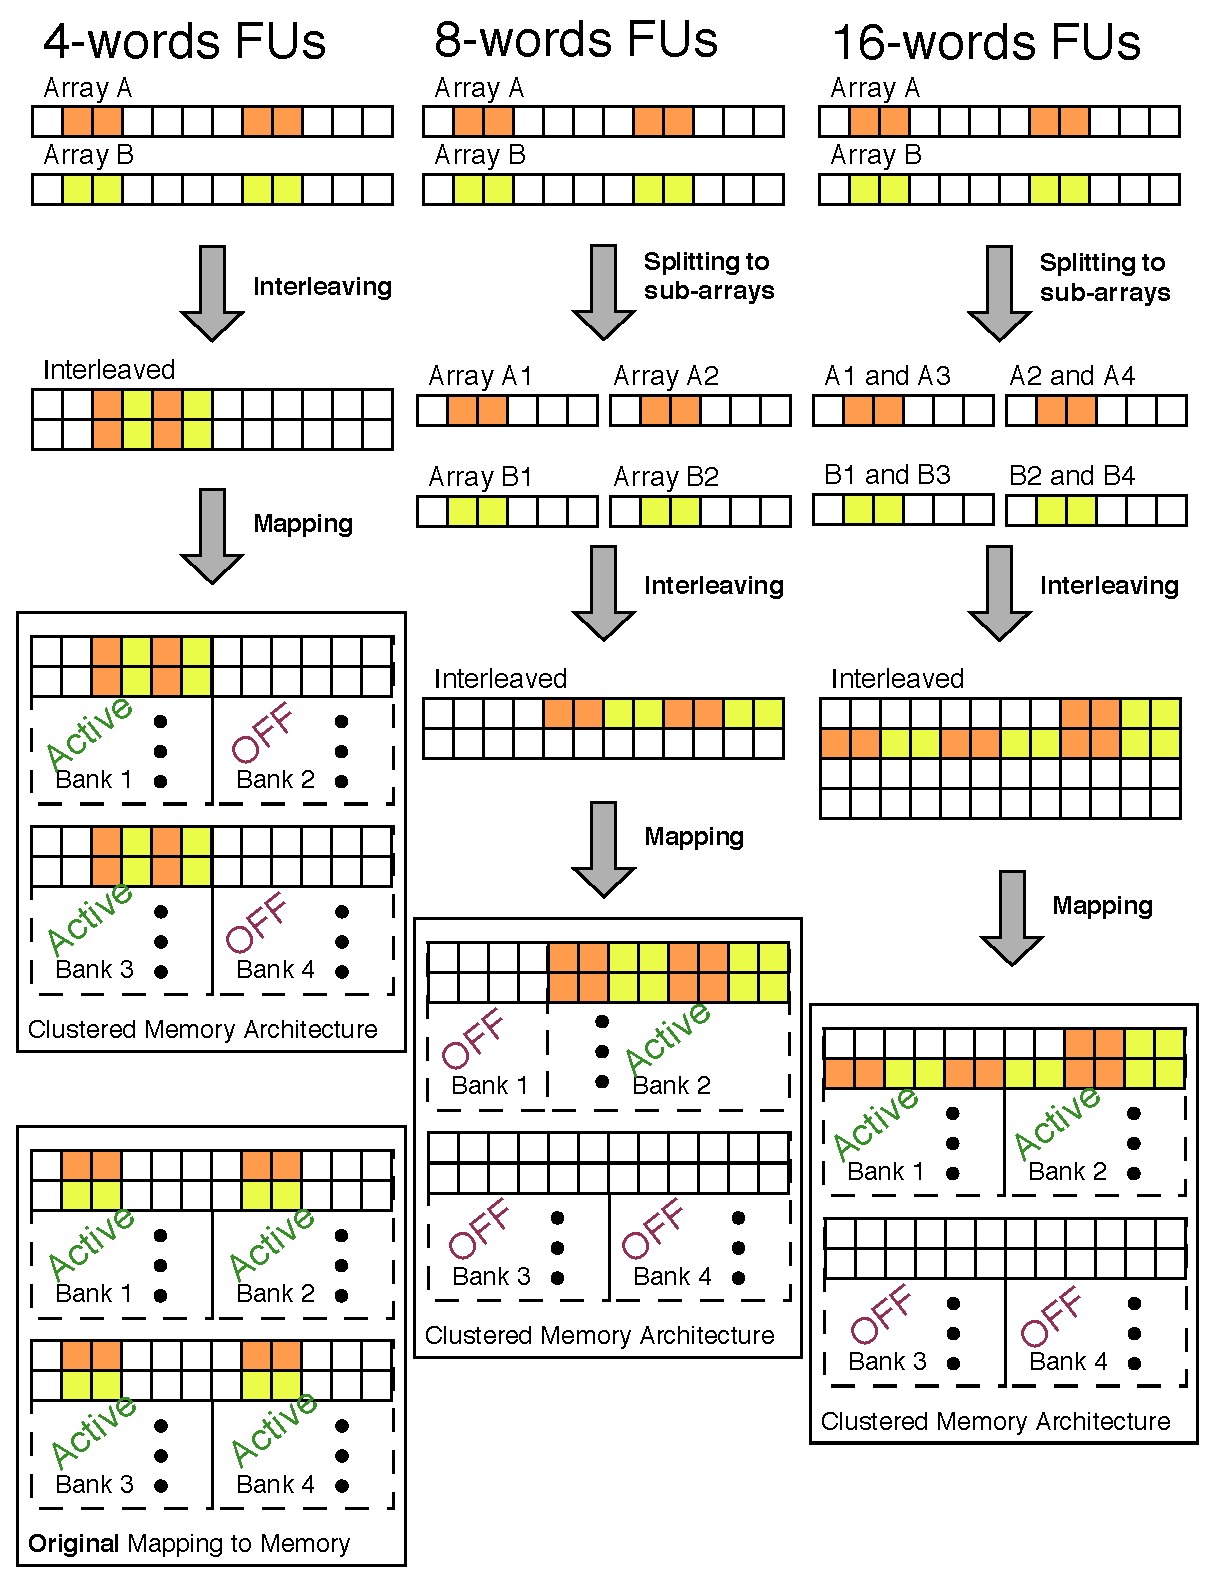
\includegraphics[width=0.45\linewidth]{Images/Example.eps} & \includegraphics[width=0.45\linewidth]{Images/sor.eps} \\
\includegraphics[width=0.45\linewidth]{Images/fft.eps} & 
\includegraphics[width=0.45\linewidth]{Images/mest.eps} 
\end{tabular}}
\end{table}


The design exploration is applied to the chosen application benchmark and energy numbers are derived based on the described target platform.
Results are presented for the four cases:
\begin{itemize}
\item No optimization
\item Interleaving exploration with a static memory platform (gain A)
\item Data mapping exploration on a reconfigurable platform without optimized interleaving (gain B)
\item Co-exploration of interleaving and mapping options (gain C, C$ > $A+B )
\end{itemize}

\section{Conclusion}

Justify why the integrated approach gives better results than just combining the two methods...
% Bibliography
\bibliographystyle{ACM-Reference-Format-Journals}
\bibliography{reference}

\end{document}